\documentclass{chi-ext}

\copyrightinfo{
  Copyright is held by the author/owner(s).\\
  \emph{CHI'12}, May 5--10, 2012, Austin, Texas, USA.\\
  ACM 978-1-4503-1016-1/12/05.\\
}

\title{Sketch It, Make It: Sketching precise drawings for laser cutting}

\numberofauthors{4}
% Notice how author names are alternately typesetted to appear ordered
% in 2-column format; i.e., the first 4 autors on the first column and
% the other 4 auhors on the second column.  Actually, it's up to you
% to strictly adhere to this author notation.
\author{
  \alignauthor{
  	\textbf{Gabe Johnson}\\
  	\affaddr{Carnegie Mellon University}\\
  	\affaddr{Pittsburgh PA}\\
  	\email{johnsogg@cmu.edu}\\
  }\alignauthor{
  	\textbf{Mark D. Gross}\\
  	\affaddr{Carnegie Mellon University}\\
  	\affaddr{Pittsburgh PA}\\
  	\email{mdgross@cmu.edu}\\
  }\\
  \\
  \\
  \alignauthor{
  	\textbf{Ellen Yi-Luen Do}\\
  	\affaddr{Georgia Inst. of Technology}\\
  	\affaddr{Atlanta GA}\\
  	\email{ellendo@gatech.edu}\\
  }%\alignauthor{
  %	\textbf{Jason I. Hong}\\
  %	\affaddr{Carnegie Mellon University}\\
  %	\affaddr{Pittsburgh PA}\\
  %	\email{jasonh@cs.cmu.edu}\\
  %}\\
}

\teaser{
  \centering
  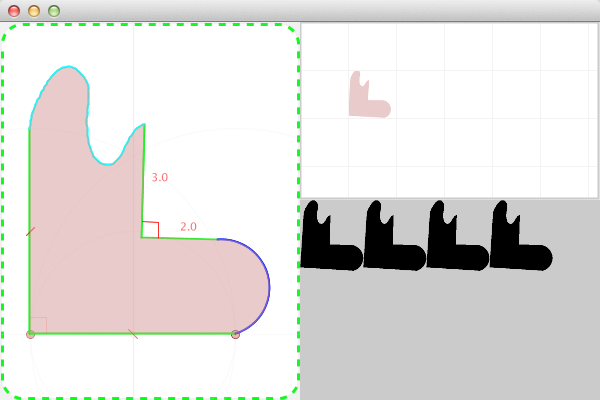
\includegraphics[width=0.87\columnwidth]{img/skruifab-full.png}
  \caption{Sketch It, Make It enables users to quickly create precise vector
    drawings like this using sketch-based interaction.}
  \label{fig:sample}
}

% Paper metadata (use plain text, for PDF inclusion and later
% re-using, if desired)
\def\plaintitle{Sketch It, Make It} 

\def\plainauthor{Gabe Johnson}

\def\plainkeywords{Sketching, Design, Constraints}

\def\plaingeneralterms{Sketching, Design, Constraints}

\hypersetup{
  % Your metadata go here
  pdftitle={\plaintitle},
  pdfauthor={\plainauthor},  
  pdfkeywords={\plainkeywords},
  pdfsubject={\plaingeneralterms},
  % Quick access to color overriding:
  citecolor=black,
  linkcolor=black,
  menucolor=black,
  urlcolor=black,
}

\usepackage{graphicx}   % for EPS use the graphics package instead
\usepackage{balance}    % useful for balancing the last columns
\usepackage{bibspacing} % save vertical space in references

% ----------------------------------------------------------------------

\begin{document}

\maketitle

\begin{abstract}
Sketch It, Make It (SIMI) is a modeling tool that enables non-experts
to design items for fabrication with laser cutters. SIMI recognizes
rough, freehand input as a user iteratively edits a structured vector
drawing. The tool combines the strengths of sketch-based interaction
with the power of constraint-based modeling. Several sketch-based
interaction techniques are combined to present a coherent system that
makes it easier to design for laser cutters.
\end{abstract}

\keywords{\plainkeywords}
% Get CHI keywords and put them here.
\category{I.3.5}{Computational Geometry and Object Modeling}{Modeling packages}


% ======================================================================
\section{Introduction}
% ======================================================================


Rapid fabrication machines such as laser cutters and 3D printers allow
people to make things that would otherwise be too difficult or time
consuming to build. Such machines are becoming more common as their
quality improves and their cost declines. Today's design/build process
typically begins with sketching on paper followed by a session with a
computer tool, and eventually, the fabrication machinery is set to
work.

\begin{figure}
\hspace*{-0.2\columnwidth}% displace figure
\parbox{\columnwidth}{
  \begin{center}
  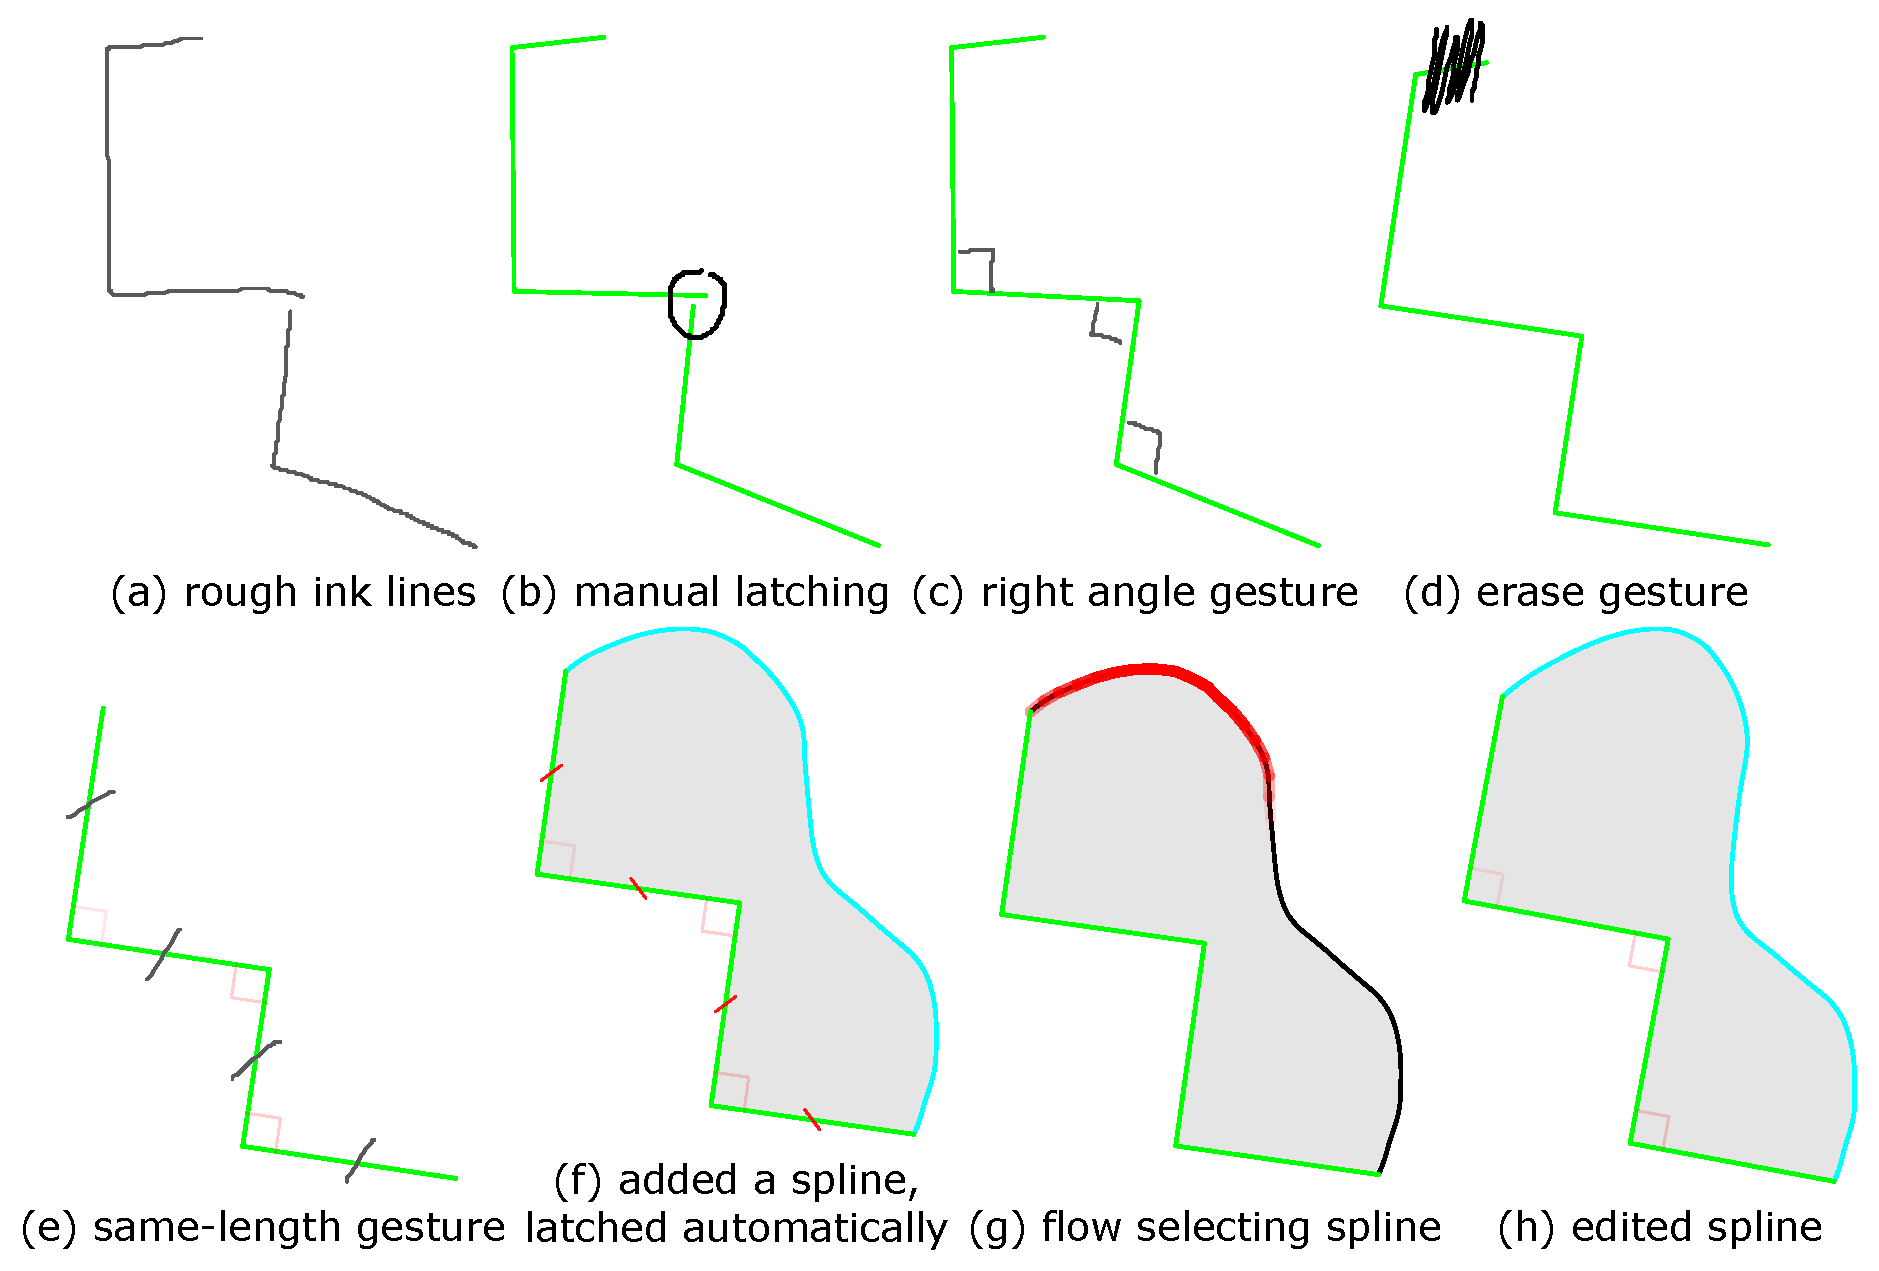
\includegraphics[width=1.2\columnwidth]{img/example-2.pdf}
  \caption{Several sketch interaction techniques for creating and
    editing structured diagrams.}
  \label{fig:bigexample}
  \end{center}  
}
\end{figure}

Unfortunately, people often have difficulty using modeling software
when designing for these machines. The system described in this paper
aims to make it easier and faster to move from idea to
specification. Observing that freehand drawing is a common way to
easily give form to ideas, we use this as a starting point for our
design tool.


% =============================================================================
\section{Sketch It, Make It (SIMI)}
% =============================================================================

SIMI presents a set of mutually cohesive sketch-based interaction
techniques for modeling items that will be produced on a laser
cutter. The guiding heuristic for developing these techniques is that
the user should never need to set down the pen. Input is provided
entirely with a stylus and a single button used with the non-dominant
hand.

Many techniques demonstrated in SIMI are inspired by other
sketch-based tools such as ParSketch~\cite{naya-parsketch} and
Lineogrammer~\cite{zeleznik-lineogrammer}. Like SIMI, those systems
supported users to iteratively build structured 2D models using sketch
input.

SIMI does not have persistent modes. Rather than requiring users to
invoke modal tools such as line, select, erase, and so on, SIMI
dynamically deduces the user's intention via recognition.

In general, the system collects rough pen input and waits for the user
to request recognition by pressing the offhand button. The first two
panes of Figure~\ref{fig:bigexample} illustrate this. In the first
pane, the designer simply adds one or more ink strokes. When the user
presses the button, SIMI attempts to recognize the designer's
intention by analyzing the most recent batch of digital ink. Here the
input was interpreted as creating line work: straight lines are green,
and the upper-right edge is a free form spline. Closed shapes are
shaded slightly, indicating complete stencils ready for laser cutting.

SIMI first segments input into primitive parts: dots, lines,
elliptical arcs, and splines. We use a segmentation and corner finding
strategy based on MergeCF~\cite{wolin-smr}. Elliptical segments may be
at any orientation, and are found using the least-squares method
described by Fitzgibbon
\textit{et. al}~\cite{fitzgibbon-ellipse-fitting}.

SIMI also recognizes commands that manipulate existing geometry
(illustrated in Figure~\ref{fig:bigexample}). All commands are
context-sensitive. For example, SIMI recognizes a right angle when it
identifies a half-square symbol near the intersection of two line
segments.

Most commands are recognized only after the button is pressed, but a
few frequently used commands are immediate. These are triggered by
gestures that are unlikely to be confused with other commands or line
work. Other commands can make use of the fact that they might comprise
several pen strokes. For example, to make two lines the same length
the user draws a short hash over each line, as shown at the lower
left. The user may hash several lines to constrain them all to be the
same length, and press the button to invoke the command.

\subsection{Latching}

\marginpar{
\begin{figure}
  \begin{center}
  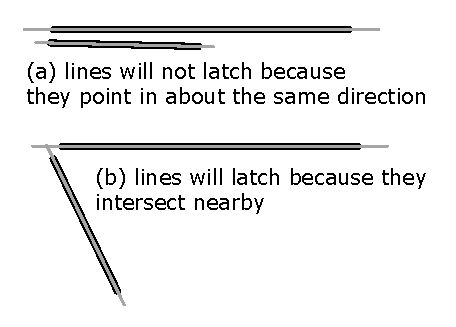
\includegraphics[width=\marginparwidth]{img/latch.pdf}
  \caption{Automatic latching depends on endpoint position, relative
    angle, and segment lengths.}
  \label{fig:latch}
  \end{center}  
\end{figure}
}

\marginpar{
\begin{figure}
  \begin{center}
  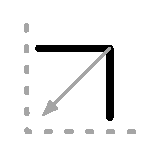
\includegraphics[width=\marginparwidth]{img/right-angle.pdf}
  \caption{Right angle gesture (dark) will be applied if (and only if)
    it is near a junction resembling the light, dashed lines.}
  \label{fig:right-angle}
  \end{center}  
\end{figure}
}

SIMI supports latching endpoints of two nearby segments. Latching can
be performed automatically or manually by user command. The system
automatically latches endpoints just after recognizing new line
work. For each newly-found segment, SIMI identifies all other segments
with nearby endpoints and forms candidate pairs. For each pair,
segment extensions are extrapolated based on the segment's type
(e.g. line or arc) (shown in light, thin lines in
Figure~\ref{fig:latch}. The extensions are 10\% of the total line
length, or 10 pixels, whichever is larger. If the two extended
segments intersect near the related endpoints, SIMI latches them.

We have implemented a way to quickly merge nearby points
manually. This technique was inspired by the lasso gesture in Bae's
EverybodyLovesSketch system~\cite{bae-everybody}. To merge nearby
endpoints, the user draws a small circle around them. This gesture is
recognized and acted upon immediately.

\subsection{Scribble Erase}

The designer removes items by scratching them out. Line work,
constraints, and unrecognized ink can all be erased. Only gestures
bigger than a certain size (100px currently) and took longer than half
a second to make are considered. The erase gesture is recognized by
computing the density of pen sample points in the gesture's convex
hull. If the density is higher than a certain threshold it is accepted
as a potential erase gesture. Next, suitable targets are sought. If
only one object is underneath the gesture's convex hull, it is
removed. If the erase gesture covers several objects, SIMI intersects
the gesture's hull with each object's hull, and computes the ratio of
the area of the intersection region with the area of the object's
hull. These ratios are clustered using k-means, and the top cluster's
objects are removed, making it possible to accurately remove small
items.

\subsection{Right Angle}

Right angles are frequently needed in laser-cut items. To make two
sketch lines perpendicular, the user draws two short lines that meet,
in the conventional `right angle' symbol. If this symbol appears near
a junction that is 90$^{\circ}$ (\pm15$^{\circ}$), the segments
composing that junction will be constrained to meet at a right angle,
as shown in Figure~\ref{fig:right-angle}. Size and context
requirements disambiguate a right angle command from
ink used to draw similarly-shaped line work.

\subsection{Same Length}

Users may instruct SIMI to make two or more segments the same length
by drawing hashes over them. This can be done in one batch (as shown
in Figure~\ref{fig:bigexample}), or in several batches by hashing
one constrained segment and one or more unconstrained segments. The
unconstrained segments are then brought into the set of related edges.

\subsection{Flow Selection}

SIMI supports lets users edit the shape of splines by using flow
selection~\cite{johnson-flow-selection}. The user briefly dwells the
pen near a spline, growing the selection area. Then, without lifting
the stylus up, the designer moves it to reshape the selected region.

\section{Constraint Engine}

Most of SIMI's commands relate to establishing geometric rules
(constraints), such as ``make this line perpendicular to that line'',
``make these three segments the same length''. SIMI's custom-built
constraint engine for 2D geometry is a numeric, iterative solver. As
constraints are added or removed, the solver repeatedly manipulates
vertices and other objects until all the constraints are satisfied, or
until it determines it can not find a solution. Sutherland used this
approach in his SketchPad system~\cite{sutherland-sketchpad}. 

\section{Future Work}

The work borrows conventions from disciplines such as mechanical
engineering and architecture. Techniques like hatching (e.g. to
indicate similar regions) deserve consideration. We are currently
exploring ways to use temporary guides (e.g. straight edges, French
curves) to aid drawing.

SIMI should also support zooming. Laser-cut items often contain small
regions that require great detail that are difficult to draw without
zooming in.

The system does not yet recognize character input for adding
dimensions to angles and lengths. For now we ``cheat'' by
allowing keyboard input. 

The custom constraint engine makes it it possible to include
additional geometry rules in the future, such as the ability to use
surface tangents.

In the near future we will begin testing SIMI with students who
regularly use laser cutters. This will help guide development.

\balance
\bibliographystyle{acm-sigchi}
\bibliography{sketch-bibliography}

\end{document}
